% Options for packages loaded elsewhere
\PassOptionsToPackage{unicode}{hyperref}
\PassOptionsToPackage{hyphens}{url}
%
\documentclass[
]{article}
\usepackage{lmodern}
\usepackage{amssymb,amsmath}
\usepackage{ifxetex,ifluatex}
\ifnum 0\ifxetex 1\fi\ifluatex 1\fi=0 % if pdftex
  \usepackage[T1]{fontenc}
  \usepackage[utf8]{inputenc}
  \usepackage{textcomp} % provide euro and other symbols
\else % if luatex or xetex
  \usepackage{unicode-math}
  \defaultfontfeatures{Scale=MatchLowercase}
  \defaultfontfeatures[\rmfamily]{Ligatures=TeX,Scale=1}
\fi
% Use upquote if available, for straight quotes in verbatim environments
\IfFileExists{upquote.sty}{\usepackage{upquote}}{}
\IfFileExists{microtype.sty}{% use microtype if available
  \usepackage[]{microtype}
  \UseMicrotypeSet[protrusion]{basicmath} % disable protrusion for tt fonts
}{}
\usepackage{xcolor}
\IfFileExists{xurl.sty}{\usepackage{xurl}}{} % add URL line breaks if available
\IfFileExists{bookmark.sty}{\usepackage{bookmark}}{\usepackage{hyperref}}
\hypersetup{
  pdftitle={Chapter 3 Results},
  pdfauthor={Meg Cychosz},
  hidelinks,
  pdfcreator={LaTeX via pandoc}}
\urlstyle{same} % disable monospaced font for URLs
\usepackage[margin=1in]{geometry}
\usepackage{longtable,booktabs}
% Correct order of tables after \paragraph or \subparagraph
\usepackage{etoolbox}
\makeatletter
\patchcmd\longtable{\par}{\if@noskipsec\mbox{}\fi\par}{}{}
\makeatother
% Allow footnotes in longtable head/foot
\IfFileExists{footnotehyper.sty}{\usepackage{footnotehyper}}{\usepackage{footnote}}
\makesavenoteenv{longtable}
\usepackage{graphicx,grffile}
\makeatletter
\def\maxwidth{\ifdim\Gin@nat@width>\linewidth\linewidth\else\Gin@nat@width\fi}
\def\maxheight{\ifdim\Gin@nat@height>\textheight\textheight\else\Gin@nat@height\fi}
\makeatother
% Scale images if necessary, so that they will not overflow the page
% margins by default, and it is still possible to overwrite the defaults
% using explicit options in \includegraphics[width, height, ...]{}
\setkeys{Gin}{width=\maxwidth,height=\maxheight,keepaspectratio}
% Set default figure placement to htbp
\makeatletter
\def\fps@figure{htbp}
\makeatother
\setlength{\emergencystretch}{3em} % prevent overfull lines
\providecommand{\tightlist}{%
  \setlength{\itemsep}{0pt}\setlength{\parskip}{0pt}}
\setcounter{secnumdepth}{5}
\usepackage{booktabs}
\usepackage{longtable}
\usepackage{array}
\usepackage{multirow}
\usepackage{wrapfig}
\usepackage{float}
\usepackage{colortbl}
\usepackage{pdflscape}
\usepackage{tabu}
\usepackage{threeparttable}
\usepackage{threeparttablex}
\usepackage[normalem]{ulem}
\usepackage{makecell}
\usepackage{xcolor}

\title{Chapter 3 Results}
\author{Meg Cychosz}
\date{12/15/2019}

\begin{document}
\maketitle

{
\setcounter{tocdepth}{2}
\tableofcontents
}
\hypertarget{results}{%
\section{Results}\label{results}}

The primary research question in this experiment asks how child and adult Quechua speakers coarticulate between and within morphemes. The results begin with descriptive statistics concerning the amount of coarticulation by age group (children aged 5 through adults) and morphological environment (within versus between morphemes). Additional descriptive statistics outline the duration of the VC sequences by age group and morphological environment. Then, a series of models are fit to predict coarticulation and duration by age and morphological environment. These models are complemented by an analysis highlighting how coarticulation interacts with duration differently in adults and children in the two morphological environments.

All analyses were conducted in the RStudio computing environment (version: 1.2.5019; rstudio, 2019). Data visualizations were created with \texttt{ggplot2} (Wickham, 2016). Modeling was conducted using the \texttt{lme4} (Bates et al., 2015), \texttt{lmerTest} (Kuznetsova et al., 2017), and \texttt{glmmTMB} (Brooks et al., 2017) packages and summaries were presented with \texttt{papaja} (Aust \& Barth, 2019) and \texttt{Stargazer} (Hlavac, 2018). Tests of residual normality were conducted using the \texttt{normtest} package (Gavrilov \& Pusev, 2014). The significance of potential model parameters was determined using a combination of log-likelihood comparisons between models, AIC estimations, and p-values procured from model summaries. In all models, continuous predictors were mean-centered to facilitate model interpretation.

\hypertarget{descriptive-statistics}{%
\subsection{Descriptive statistics}\label{descriptive-statistics}}

\hypertarget{coarticulation}{%
\subsubsection{Coarticulation}\label{coarticulation}}

The degree of coarticulation between the VC sequences {[}ap{]} and {[}am{]} was measured using the spectral distance metric described in experiment one For this coarticulation metric, coarticulation is quantified as the Euclidean distance between the spectral vectors of two adjacent phones, henceforth the Mel spectral distance. In this outcome measure, a larger spectral distance between phones equates to \emph{less} coarticulation between the phones.

\begin{table}

\caption{\label{tab:ap-coartic-tbl}Mean spectral distance between [a] and [p] by age and word position}
\centering
\begin{tabular}[t]{lrrrr}
\toprule
\multicolumn{1}{c}{ } & \multicolumn{2}{c}{Across boundary} & \multicolumn{2}{c}{Within boundary} \\
\cmidrule(l{3pt}r{3pt}){2-3} \cmidrule(l{3pt}r{3pt}){4-5}
Age & Spectral\_Distance  & SD  & Spectral\_Distance & SD\\
\midrule
5 & 17.42 & 4.64 & 19.63 & 4.56\\
6 & 17.62 & 4.70 & 19.78 & 4.59\\
7 & 17.04 & 4.68 & 19.18 & 5.90\\
8 & 18.50 & 6.03 & 21.35 & 6.76\\
9 & 16.21 & 7.02 & 17.51 & 7.79\\
\addlinespace
10 & 14.92 & 5.09 & 15.93 & 5.07\\
adult & 14.99 & 3.64 & 14.51 & 3.03\\
\bottomrule
\end{tabular}
\end{table}

\begin{table}

\caption{\label{tab:am-coartic-tbl}Mean spectral distance between [a] and [m] by age and word position}
\centering
\begin{tabular}[t]{lrrrr}
\toprule
\multicolumn{1}{c}{ } & \multicolumn{2}{c}{Across boundary} & \multicolumn{2}{c}{Within boundary} \\
\cmidrule(l{3pt}r{3pt}){2-3} \cmidrule(l{3pt}r{3pt}){4-5}
Age & Spectral\_Distance  & SD  & Spectral\_Distance & SD\\
\midrule
5 & 7.94 & 3.13 & 8.71 & 3.39\\
6 & 8.44 & 3.08 & 9.54 & 4.76\\
7 & 8.43 & 3.11 & 8.86 & 3.80\\
8 & 9.89 & 3.99 & 9.73 & 3.78\\
9 & 7.43 & 2.64 & 8.06 & 3.11\\
\addlinespace
10 & 8.21 & 3.43 & 8.30 & 4.25\\
adult & 7.44 & 4.19 & 7.00 & 3.34\\
\bottomrule
\end{tabular}
\end{table}

Table \ref{tab:ap-coartic-tbl} shows the mean Mel spectral distance between the segments in {[}ap{]} (words inflected with \emph{-pi} for the across morpheme boundary condition) and Table \ref{tab:am-coartic-tbl} shows this for {[}am{]} (words inflected with \emph{-man} for the across morpheme boundary condition). Unsurprisingly, there is a larger average spectral distance between the vowel and plosive in {[}ap{]} than the vowel and nasal in {[}am{]} because the segments in {[}am{]} have increased acoustic similarity (sonority, voicing). Next, looking by age group for coarticulation between {[}ap{]}, it is apparent that the amount of coarticulation between segments increases as children age. This is likely due to the increased speaking rate in the older cohorts and adults, as will become apparent when these results are crossed with sequence duration. There is less within age group variability in {[}ap{]} productions in the adult speakers as well (reflected in the smaller SD of the mean for the adults). Variability does not appear to decrease linearly as both the nine and ten-year-old cohorts exhibit larger SDs than the five and six-year-olds. However, this could also reflect the smaller sample sizes in the older cohorts (5 ten-year-olds and 5 nine-year-olds but 10 each in the five- and six-year-old cohorts).

For the coarticulation patterns between segments in {[}am{]}, adults and children appear to coarticulate similarly, irrespective of age group. There is slightly greater variability in the amount of coarticulation (larger SD) in the adult group. Overall, the difference in developmental coarticulatory patterns between the VC sequence {[}am{]} and the sequence {[}ap{]} could be due to differences in the \emph{-man} suffix use in Quechua (frequency, productivity). Alternatively, differences between these sequences could be due to the acoustic differences between {[}ap{]} and {[}am{]} as segments in {[}am{]} are more acoustically similar than segments in {[}ap{]}.

\hypertarget{duration}{%
\subsubsection{Duration}\label{duration}}

We next turned to descriptive statistics describing the interaction of coarticulation and sequence duration. Duration could interact with coarticulation, and age, as speakers coarticulate more in fast speech (Gay, 1981), and adults speak faster than children (Lee et al., 1999).

\begin{table}

\caption{\label{tab:ap-dur-tbl}Mean duration of [ap] sequence by age and word position}
\centering
\begin{tabular}[t]{lrrrr}
\toprule
\multicolumn{1}{c}{ } & \multicolumn{2}{c}{Across boundary} & \multicolumn{2}{c}{Within boundary} \\
\cmidrule(l{3pt}r{3pt}){2-3} \cmidrule(l{3pt}r{3pt}){4-5}
Age & Duration (ms) & SD  & Duration (ms) & SD\\
\midrule
5 & 228.7 & 47 & 339.9 & 52\\
6 & 242.5 & 45 & 334.4 & 59\\
7 & 245.1 & 57 & 319.8 & 60\\
8 & 226.9 & 56 & 329.3 & 43\\
9 & 216.6 & 36 & 312.6 & 56\\
\addlinespace
10 & 212.8 & 50 & 302.3 & 63\\
adult & 205.7 & 47 & 197.0 & 59\\
\bottomrule
\end{tabular}
\end{table}

\begin{table}

\caption{\label{tab:am-dur-tbl}Mean duration of [am] sequence by age and word position}
\centering
\begin{tabular}[t]{lrrrr}
\toprule
\multicolumn{1}{c}{ } & \multicolumn{2}{c}{Across boundary} & \multicolumn{2}{c}{Within boundary} \\
\cmidrule(l{3pt}r{3pt}){2-3} \cmidrule(l{3pt}r{3pt}){4-5}
Age & Duration (ms) & SD  & Duration (ms) & SD\\
\midrule
5 & 214.4 & 45 & 251.2 & 66\\
6 & 217.9 & 58 & 247.8 & 62\\
7 & 209.8 & 42 & 244.6 & 60\\
8 & 218.2 & 63 & 247.1 & 53\\
9 & 199.8 & 30 & 231.8 & 64\\
\addlinespace
10 & 194.3 & 33 & 239.9 & 57\\
adult & 175.6 & 36 & 173.7 & 39\\
\bottomrule
\end{tabular}
\end{table}

Table \ref{tab:ap-dur-tbl} maps average sequence duration of {[}ap{]} by age and word position and Table \ref{tab:am-dur-tbl} does similarly for {[}am{]}. Overall, duration of {[}ap{]} decreases with age, with adult speakers exhibiting the shortest average duration for {[}ap{]} for both word positions. Of note is that the average duration of {[}ap{]} sequences within morphemes tended to be longer than the duration of {[}ap{]} sequences across boundaries for all of the children. This pattern was reversed in the adult speakers, however, whose average {[}ap{]} duration within morpheme boundaries was actually \emph{shorter} than across. This pattern will be revisited in the modelling portion of the Results.

Turning to the sequence {[}am{]}, the average duration of the {[}am{]} sequence in adult speakers was shorter than all of the child speakers; and like {[}ap{]}, {[}am{]} duration also appears to decrease with age. This pattern of {[}am{]} duration decreasing with age is consistent for both word positions, across and within morphemes.

Concerning differences by word position, all age groups showed, on average, shorter {[}am{]} durations in the across morpheme condition, contrary to the finding that {[}ap{]} sequence duration was longer in the across morpheme condition for adults. However, it is important to note the average duration of {[}am{]} by word position in adults only differed by approximately 3 ms while the average within morpheme condition in children was approximately 40 ms greater than the across morpheme condition in children. Thus, for both {[}am{]} and {[}ap{]} sequences, there appears to be a difference in sequence duration by word position for adult and child speakers. In the following section we turn to the modeling of coarticulation before illustrating how degree of coarticulation interacts with duration differently in the adults and children.

\hypertarget{modelling-interaction-of-coarticulation-and-duration}{%
\subsection{Modelling interaction of coarticulation and duration}\label{modelling-interaction-of-coarticulation-and-duration}}

The central research question in this study asked if child and adult Quechua speakers would coarticulate similarly between VC sequences across versus within morpheme boundaries. To answer this question, a series of generalized linear mixed effect models (GLMMs) were fit to predict degree of coarticulation (Mel spectral distance between each V and C). GLMMs were chosen instead of the more common linear mixed effect models due to the non-normality of the residual \textbf{VC Sequence duration} (henceforth simply \textbf{Sequence Duration}) which was included in all models. (Shapiro tests of kurtosis and skewness for \textbf{Sequence duration} indicated that we could reject the null hypothesis that the residual's distribution did not differ significantly from a normal distribution. Kurtosis t=5.53, p\textless.001 and skewness: t=1.07, p\textless.001 {[}Shapiro et al., 1968{]}.) Specifically, the response variable \textbf{Spectral distance} and the residual \textbf{Sequence duration} are both limited to non-negative values (as all VC sequences had some distance between the V and C and all had a duration), with a resultant right skew to the data distribution.

The choice to fit gamma GLMMs, as opposed to log-normalizing \textbf{Sequence duration} and fitting linear mixed models, reflects recent suggestions in cognitive psychology to avoid data transformation, even for commonly-transformed variables such as time/duration, in an effort to facilitate between-study comparison (Lo \& Andrews, 2015). Consequently, gamma GLMMs were fit using a log linking function to appropriately model the skewed, non-Gaussian distribution of the residual.

A GLMM was fit to predict the spectral distance between segments in the VC sequences. Baseline models included random effects of \textbf{Participant} and \textbf{Word} (models with random slopes of \textbf{Participant} by \textbf{Word} did not converge, possibly due to the number of repetitions per speaker; see Methods). Model building then began in a forward-testing manner with predictors added in the following order: \textbf{Sequence duration}, \textbf{VC sequence} ({[}ap{]} or {[}am{]}), \textbf{Age} (adult or child), \textbf{Environment} ({[}within morpheme or between morphemes{]}), and interactions. The best model fit included the four-variable interaction of \textbf{Sequence duration}, \textbf{VC sequence}, \textbf{Age}, and \textbf{Environment}. The summary for the model containing adults and children together is included in listed in Appendix D. This four-variable interaction indicates that the coarticulation and duration patterns differ between adults and children. Consequently, given the difficulty in interpreting four-variable interactions, separate models were fit for adults and children to facilitate coefficient interpretation.

For both the adult and child groups, models were fit to predict the spectral distance between segments in the VC sequences. Best model fit for the adult and child models included the three-variable interaction of \textbf{Sequence duration}, \textbf{VC sequence}, and \textbf{Environment}: the improvement of models with this interaction over models with the three independent effects was significant for the adult model with alpha level \textless.05 (\(\chi\)\textsuperscript{2} = 12.69, df=7,11 p=.01) and the child model (\(\chi\)\textsuperscript{2} = 15.18, df=7,11, p=.004). Throughout the results, the children's patterns are additionally broken apart by age to view differences between age groups. However, note that in the child model, the addition of the variable \textbf{Age Group} (levels: 5, 6, 7, 8, 9, 10) did not improve upon a model with the interaction of \textbf{Sequence duration}, \textbf{VC sequence}, and \textbf{Environment}. This fact suggests that the pattern of coarticulation and duration by morphological environment did not significantly vary by the child's age group.

The final child model summary is listed in table \ref{tab:child-model-sum} and the adult model summary is listed in table \ref{tab:adult-model-sum}. Note that in the model summaries for the children and adults, the coefficients and standard error measurements were multiplied by 100 to make the otherwise small coefficients more interpretable. This step does not effect the direction or magnitude of the effect between predictors and outcome variables.

\begin{table}[tbp]

\begin{center}
\begin{threeparttable}

\caption{\label{tab:adult-model-sum}Model predicting coarticulation in adults}

\begin{tabular}{llllll}
\toprule
term & \multicolumn{1}{c}{estimate} & \multicolumn{1}{c}{S.E.} & \multicolumn{1}{c}{z.statistic} & \multicolumn{1}{c}{p.value} & \multicolumn{1}{c}{95\% CI}\\
\midrule
Intercept & 213.56 & 5.50 & 38.84 & 0.00 & 2.24,2.03\\
Sequence duration & 0.33 & 0.06 & 5.52 & 0.00 & 0,0\\
Environment:across morpheme & -7.56 & 6.89 & -1.10 & 0.27 & 0.06,-0.21\\
VC sequence:ap & 61.78 & 5.73 & 10.78 & 0.00 & 0.73,0.51\\
Sequence duration*Environment:across morpheme & -0.22 & 0.08 & -2.88 & 0.00 & 0,0\\
Sequence duration*VC sequence:ap & -0.21 & 0.07 & -2.95 & 0.00 & 0,0\\
Environment:across morpheme*VC sequence:ap & 6.80 & 8.05 & 0.84 & 0.40 & 0.23,-0.09\\
Sequence duration*Environment:across morpheme*VC sequence:ap & 0.29 & 0.09 & 3.20 & 0.00 & 0,0\\
\bottomrule
\end{tabular}

\end{threeparttable}
\end{center}

\end{table}

\begin{table}[tbp]

\begin{center}
\begin{threeparttable}

\caption{\label{tab:child-model-sum}Model predicting coarticulation in children}

\begin{tabular}{llllll}
\toprule
term & \multicolumn{1}{c}{estimate} & \multicolumn{1}{c}{S.E.} & \multicolumn{1}{c}{z.statistic} & \multicolumn{1}{c}{p.value} & \multicolumn{1}{c}{95\% CI}\\
\midrule
Intercept & 216.80 & 3.70 & 58.66 & 0.00 & 2.24,2.1\\
Sequence duration & 0.06 & 0.02 & 3.15 & 0.00 & 0,0\\
Environment:across morpheme & -0.94 & 3.33 & -0.28 & 0.78 & 0.06,-0.07\\
VC sequence:ap & 72.39 & 4.44 & 16.32 & 0.00 & 0.81,0.64\\
Sequence duration*Environment:across morpheme & 0.07 & 0.03 & 2.38 & 0.02 & 0,0\\
Sequence duration*VC sequence:ap & -0.01 & 0.03 & -0.32 & 0.75 & 0,0\\
Environment:across morpheme*VC sequence:ap & -6.06 & 5.08 & -1.19 & 0.23 & 0.04,-0.16\\
Sequence duration*Environment:across morpheme*VC sequence:ap & -0.09 & 0.04 & -2.40 & 0.02 & 0,0\\
\bottomrule
\end{tabular}

\end{threeparttable}
\end{center}

\end{table}

In the adult and child models, a positive coefficient for the predictor \textbf{VC sequence}, with the reference level `{[}ap{]}', shows that there was greater spectral distance between the segments in {[}ap{]} than {[}am{]}, as we would anticipate given the acoustic signatures of {[}m{]} (voiced, sonorant) versus {[}p{]} (voiceless, transient) (adult model: \(\beta\)=61.78, z=10.78, p\textless.001; child model: \(\beta\)=72.39, z=16.32, p\textless.001).

Also of note in both the adult and child models is the direction of the \textbf{Sequence duration} predictor: a positive coefficient for \textbf{Sequence duration} indicates that longer duration VC sequences tended to also be less coarticulated (greater spectral distance between phones) (child model: \(\beta\)=0.06, z=3.15, p=0.002; adult model: \(\beta\)=0.33, z=5.52, p\textless.001). The coefficients suggest that when speakers, both adults and children alike, speak slower, they tend to coarticulate less. There is, however, an interaction between several of these predictors, which will demonstrate that children in particular do not always coarticulate less in longer-duration sequences. The direction of the interaction between \textbf{Sequence duration}, \textbf{VC sequence}, and \textbf{Environment} differs between the adult and child speakers so this will be interpreted separately for the two groups in the following section.

~
~

\begin{figure}
\centering
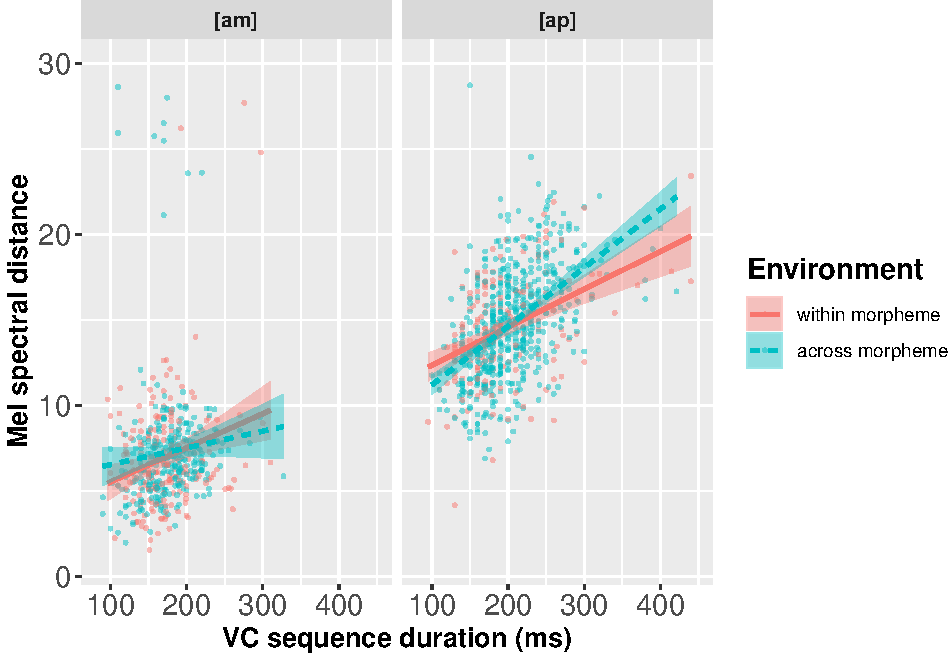
\includegraphics{3_ch3_results_files/figure-latex/adult-int-plot-1.pdf}
\caption{\label{fig:adult-int-plot}Coarticulation within VC sequence by sequence duration and morphological environment in adult speakers}
\end{figure}

\begin{figure}
\centering
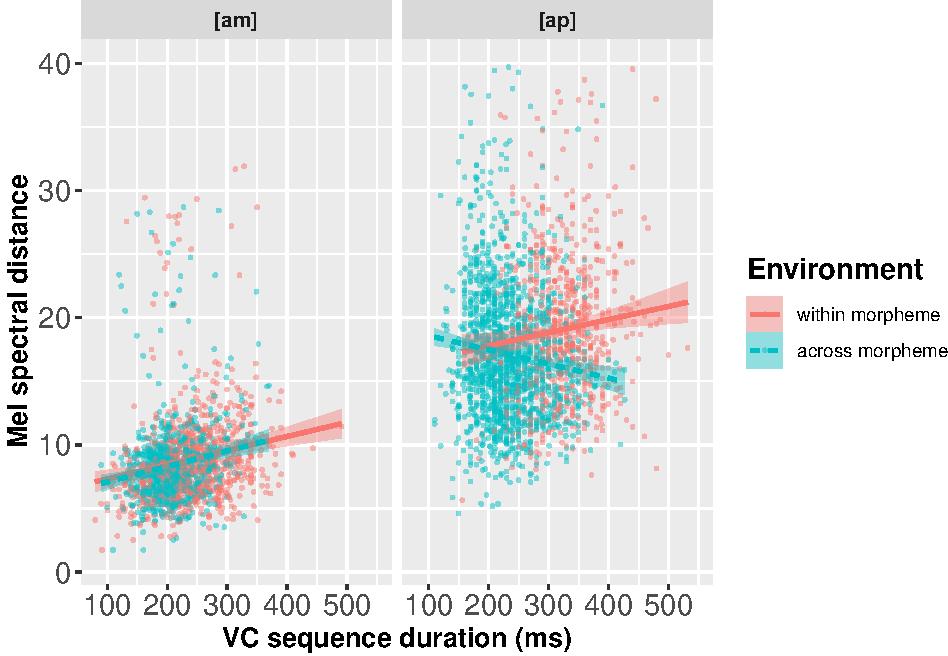
\includegraphics{3_ch3_results_files/figure-latex/child-int-plot-1.pdf}
\caption{\label{fig:child-int-plot}Coarticulation within VC sequence by sequence duration and morphological environment in all child speakers}
\end{figure}

\hypertarget{adults}{%
\subsubsection{Adults}\label{adults}}

For the adult model, the interaction between \textbf{Sequence duration}, \textbf{VC sequence}, and \textbf{Environment} suggests a difference in the relationship between the response variable - amount of coarticulation - and \textbf{Sequence duration} that differs by \textbf{Environment} and \textbf{VC sequence}. As Figure \ref{fig:adult-int-plot} demonstrates, this difference by \textbf{Environment} is apparent in the steepness of the slope for the `across morpheme' and `within morpheme' conditions for {[}am{]} and {[}ap{]}. To quantify this difference for the sequence {[}am{]}, the slopes of the two conditions were calculated. As the {[}am{]} panel in Figure \ref{fig:adult-int-plot} suggests, the slope for the `within morpheme' condition was steeper (2.14) than the slope for the `across morpheme' condition (2.06),\footnote{To reflect the data visualizations, these slopes were calculated on the beta coefficients before the coefficients were scaled by 100.} suggesting a different relationship between duration and coarticulation between the two word environments in adults.

Overall, the significance of the interaction \textbf{Sequence duration}, \textbf{VC sequence}, and \textbf{Environment} in adult speakers shows two important results: first, adults distinguish by word environment, both for {[}ap{]} versus {[}a\#p{]} sequences and {[}am{]} versus {[}a\#m{]} sequences. Second, complicating this finding, is the fact that adults distinguish between word environments differently depending upon the VC sequence. For {[}ap{]}, though adults coarticulate roughly equally across and within morphemes, the relationship between duration and coarticulation (longer duration equates to less coarticulation) is stronger in the `across morpheme' condition. For {[}am{]}, adults also distinguish between the two morphological environments by the relationship of VC duration and coarticulatory degree, but the effect of condition is reversed: the relationship between duration and coarticulation is stronger for the `within morpheme' condition.

Thus, returning to one part of the central research question - does adult coarticulation differ by word environment - we find that adults do coarticulate differently in the two word environments. However, despite these significant differences, there was nevertheless a positive relationship between duration and amount of coarticulation for all combinations of VC sequences and word environments. Adults consistently coarticulate less in longer-duration sequences. This result suggests that adult speakers may have one overarching articulatory plan for all environments and both VC sequences measured. The following section demonstrates how this relationship between duration and coarticulation may not be uniform between adults and children.

\hypertarget{children}{%
\subsubsection{Children}\label{children}}

Turning to the child model, the significant interaction of \textbf{Sequence duration}, \textbf{VC sequence}, and \textbf{Environment} suggests that children do not coarticulate similarly in longer-duration sequences for all combinations of \textbf{Environment} and \textbf{VC sequence} (Figure \ref{fig:child-int-plot}). Specifically, for {[}ap{]} sequences that occur across morpheme boundaries, the negative slope indicates that children actually coarticulate \emph{more} in longer duration sequences. The positive slope for the within morpheme boundary condition suggests that children coarticulate less in longer-duration sequences, in line with all of the adult patterns. So, children coarticulate more between segments at morpheme boundaries in words inflected with the locative marker \emph{-pi} than between those same segments that occur within morphemes.

\begin{figure}
\centering
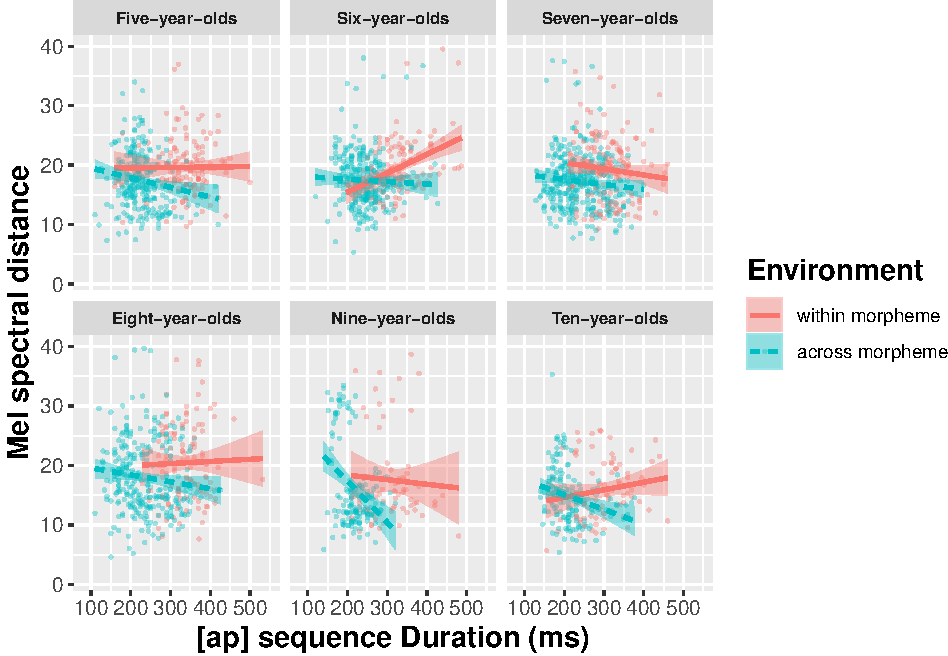
\includegraphics{3_ch3_results_files/figure-latex/child-facet-ap-1.pdf}
\caption{\label{fig:child-facet-ap}Coarticulation within {[}ap{]} by sequence duration, morphological environment, and age in child speakers}
\end{figure}

Note that this negative relationship between duration and coarticulation is counter to the positive relationship for every combination of VC sequence and word environment in adult speakers. Adults consistently coarticulate less in longer-duration sequences regardless of environment or VC sequence. The facet plot in Figure \ref{fig:child-facet-ap} plots this relationship between duration and coarticulation for {[}ap{]} for each age group (5-10 years) to ensure a consistent pattern across the groups. (Again the predictor \textbf{Age Group}, with the levels 5, 6, 7, 8, 9, and 10 years, did not improve upon the child model fit.) All age groups show the same negative relationship: the longer the {[}ap{]} sequence, the more the children coarticulate between {[}a{]} and {[}p{]} in the across morpheme condition.

\begin{figure}
\centering
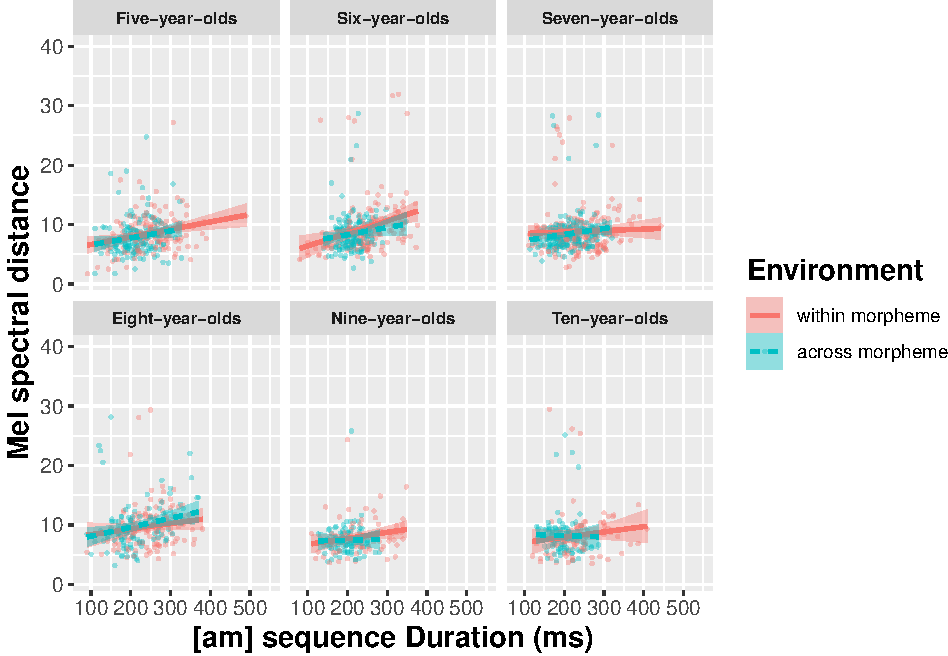
\includegraphics{3_ch3_results_files/figure-latex/child-facet-am-1.pdf}
\caption{\label{fig:child-facet-am}Coarticulation within {[}am{]} by sequence duration, morphological environment, and age in child speakers}
\end{figure}

The results for {[}am{]} in children demonstrate broadly similar results to the adult speakers: children coarticulate less between segments in longer-duration {[}am{]} sequences. The facet plot in Figure \ref{fig:child-facet-am} once again shows a similar effect for each age group. Given the between-subject variability that typically characterizes child speech, these patterns by environment are further broken apart by individual child for each age group (age 5-10) (Appendix B) to ensure no large outliers with regards to the patterning by word environment. The results by are broadly similar across speakers.

~
~

\hypertarget{interim-discussion}{%
\subsection{Interim discussion}\label{interim-discussion}}

Comparing between the adult and child models, several preliminary conclusions can be made. First, responding to the original research question - do adults and children coarticulate differently within versus between morpheme boundaries - we find that both adults and children differentiate by morphological environment. However, they do so in different ways. Adults have a single plan for both environments, and even both VC sequences: adults coarticulate less in longer-duration sequences, and overall, they coarticulate less between {[}a{]} and {[}p{]} within morphemes than across morpheme boundaries. The stark difference between adults and children emerges in the {[}ap{]} sequence patterning. Children differentiate between morphological environments via the relationship between duration and coarticulation as they coarticulate more in longer-duration sequences across morpheme boundaries and coarticulate \emph{less} in longer-duration sequences within morphemes.

For words inflected with \emph{-man}, children show a similar pattern to adults, though children do not differentiate by environment coarticulatorily. Rather, across morpheme sequences are shorter in duration than within morpheme sequences for the children. On the basis of these results, two questions remain. First, why do children differentiate between environments via a combination of duration and coarticulation; specifically, why do children produce shorter duration VC sequences across morpheme boundaries and longer duration sequences within morphemes? Second, why do children coarticulate more in longer-duration {[}ap{]} sequences that cross morpheme boundaries (e.g.~\emph{llama-pi} `llama-\textsc{loc}')? All of the other combinations of morphological environment and VC sequence in the adults and children suggest that the speakers coarticulate less in longer-duration segments.

The finding that children produce shorter-duration VC sequences in the `across morpheme' condition than the `within morpheme' condition for {[}am{]} and {[}ap{]} could be explained by a confound in word size and morphological environment. Coarticulation for the `across morpheme' condition was, necessarily, measured across morphemes. However, to derive an across morpheme environment in Quechua, nouns are inflected with suffixes (e.g.~\emph{llama} `llama' -\textgreater{} \emph{llama-pi} `llama-\textsc{loc}'). As a result, almost all of the stimuli in the `across morpheme' condition are at least one syllable longer in length than the stimuli for the `within morpheme' condition. For example, coarticulation between {[}ap{]} was frequently measured within two syllable base roots (e.g.~\emph{llapa} `lightening' and \emph{llama} `llama'). However, for the `across morpheme' condition, {[}ap{]} coarticulation was frequently measured in three-syllable inflections of these nouns (e.g.~\emph{llapa-pi} `lightening-LOC' and \emph{llama-pi} `llama-\textsc{loc}'). Even for prosodically longer words where within morpheme coarticulation was measured, such as the three-syllable \emph{hampiri} `healer' and \emph{hatun mama} `grandmother', there were equivalent across morpheme stimuli that were one syllable longer (e.g.~\emph{hatun mama-mang} `grandmother-\textsc{all}').

\hypertarget{compensatory-shortening}{%
\subsection{Compensatory shortening}\label{compensatory-shortening}}

To explore the possibility that durational differences between the `across morpheme' and `within morpheme' conditions could be due to word length, an exploratory analysis was conducted. We anticipated that sequence duration would shorten in words with more syllables, regardless of morphological context. This well-known tendency for segment durations to shorten in longer-duration/polysyllabic words is known as \textsc{Compensatory Shortening} (Harrington et al., 2015; Lehiste 1972; Munhall et al., 1992). To illustrate how this unfolds in the children's speech production for the current study, Figure \ref{fig:compshort-kids} plots VC sequence duration by the number of syllables for the children and Figure \ref{fig:compshort-adults} plots duration as a function of number of syllables for the adults. As the children's figure demonstrates, children's VC sequences are consistently shorter in words with more syllables, most notably between two- and three-syllable words. The same pattern is not apparent in the adult data: adults have fairly similar sequence lengths regardless of the number of syllables in the word (see Table \ref{tab:dur-by-syll-kids} for descriptive statistics of duration by word length in syllables for the children and Table \ref{tab:dur-by-syll-adults} for duration by word length results for the adults).

\begin{figure}
\centering
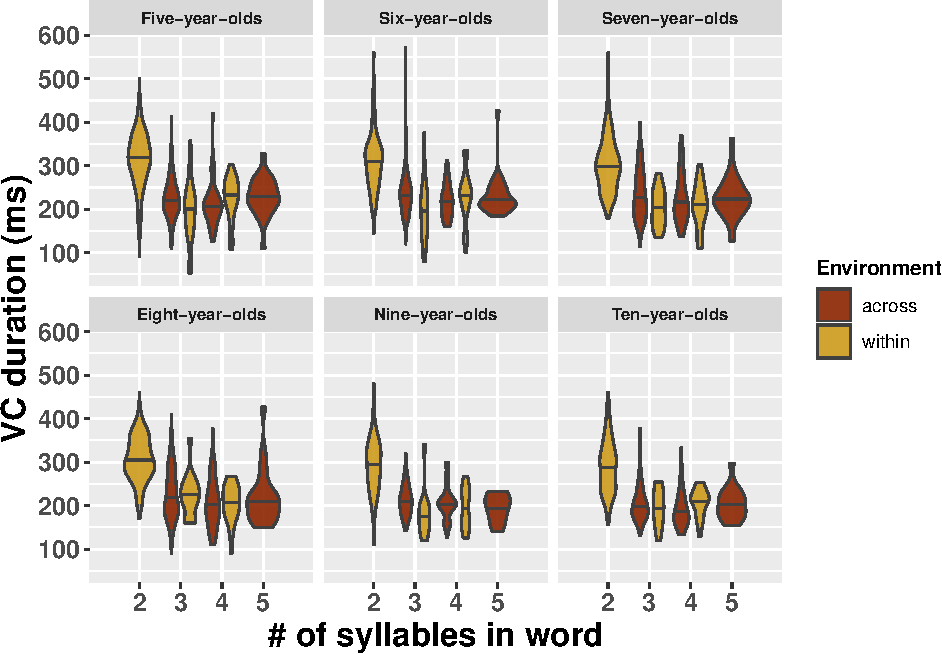
\includegraphics{3_ch3_results_files/figure-latex/compshort-kids-1.pdf}
\caption{\label{fig:compshort-kids}Sequence duration by word length and word environment: Children}
\end{figure}

\begin{figure}
\centering
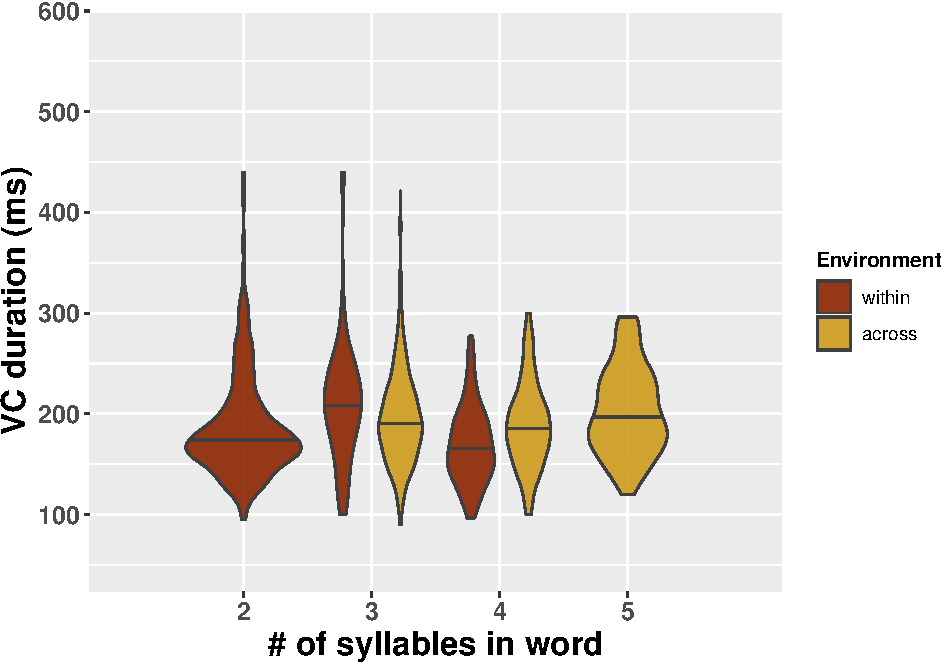
\includegraphics{3_ch3_results_files/figure-latex/compshort-adults-1.pdf}
\caption{\label{fig:compshort-adults}Sequence duration by word length and word environment: Adults}
\end{figure}

\begin{table}

\caption{\label{tab:dur-by-syll-kids}Mean VC sequence duration by number of syllables in word for children}
\centering
\begin{tabular}[t]{lrrrr}
\toprule
\multicolumn{1}{c}{ } & \multicolumn{2}{c}{[am]} & \multicolumn{2}{c}{[ap]} \\
\cmidrule(l{3pt}r{3pt}){2-3} \cmidrule(l{3pt}r{3pt}){4-5}
Syllables & Duration (ms) & SD  & Duration (ms) & SD\\
\midrule
2 & 272.9 & 52 & 325.3 & 57\\
3 & 211.6 & 51 & 235.2 & 51\\
4 & 207.6 & 46 & 220.7 & 51\\
5 & 204.1 & 35 & 230.4 & 51\\
\bottomrule
\end{tabular}
\end{table}

\begin{table}

\caption{\label{tab:dur-by-syll-adults}Mean VC sequence duration by number of syllables in word for adults}
\centering
\begin{tabular}[t]{lrrrr}
\toprule
\multicolumn{1}{c}{ } & \multicolumn{2}{c}{[am]} & \multicolumn{2}{c}{[ap]} \\
\cmidrule(l{3pt}r{3pt}){2-3} \cmidrule(l{3pt}r{3pt}){4-5}
Syllables & Duration (ms) & SD  & Duration (ms) & SD\\
\midrule
2 & 177.6 & 39 & 192.4 & 57\\
3 & 176.5 & 35 & 210.0 & 50\\
4 & 168.0 & 36 & 195.3 & 43\\
5 & 178.5 & 51 & 207.3 & 40\\
\bottomrule
\end{tabular}
\end{table}

\begin{table}[!htbp] \centering 
  \caption{Model predicting VC duration: children} 
  \label{} 
\begin{tabular}{@{\extracolsep{5pt}}lc} 
\\[-1.8ex]\hline 
\hline \\[-1.8ex] 
 Intercept & 289.36$^{***}$ \\ 
  & (276.14, 302.58) \\ 
  & \\ 
 Three syllables & $-$79.68$^{***}$ \\ 
  & ($-$90.37, $-$68.99) \\ 
  & \\ 
 Four syllables & $-$93.38$^{***}$ \\ 
  & ($-$107.40, $-$79.37) \\ 
  & \\ 
 Five syllables & $-$87.01$^{***}$ \\ 
  & ($-$108.68, $-$65.34) \\ 
  & \\ 
 VC sequence:[ap] & 27.66$^{***}$ \\ 
  & (19.56, 35.77) \\ 
  & \\ 
\hline \\[-1.8ex] 
Observations & 3,877 \\ 
Log Likelihood & $-$20,122.98 \\ 
Akaike Inf. Crit. & 40,261.97 \\ 
Bayesian Inf. Crit. & 40,312.07 \\ 
\hline 
\hline \\[-1.8ex] 
\textit{Note:}  & \multicolumn{1}{r}{$^{*}$p$<$0.05; $^{**}$p$<$0.01; $^{***}$p$<$0.001} \\ 
\end{tabular} 
\end{table}

To further explore the phenomenon of Compensatory Shortening in the children's speech, a linear mixed effects model was fit to predict the VC sequence duration in the children's speech (no skewed/non-negative predictors were included in the modelling so GLMMs were not necessary). Model fitting occurred as before in a forward-testing manner: the base model contained random effects of individual \textbf{Child} and \textbf{Word} (random slopes of Speaker by Word did not converge). Then, parameters were added in the following order: \textbf{Age} (5-10), \textbf{Number of Syllables} (2-5), \textbf{Environment} (across versus within), the interaction of \textbf{Number of Syllables} and \textbf{Environment}, and \textbf{VC sequence}. Only the predictors \textbf{Number of Syllables} and \textbf{VC sequence} improved baseline model fit (see Table \ref{tab:dursum} for model summary).

In the model summary, the positive beta coefficient for VC sequence with a reference level {[}am{]} indicates that the {[}ap{]} sequence was significantly longer than {[}am{]} sequences (as previous models demonstrated). Next, the negative beta coefficients for \textbf{Syllable Count} with a reference level of `2 syllables' indicated that VC sequence duration was approximately 80 ms shorter in three syllable words than two syllable (\(\beta\)=-79.68, t=-14.61, p\textless.001). Similarly, VC sequences were approximately 93 ms shorter in four syllable words than two syllable (\(\beta\)=-93.38, t=-13.06, p\textless.001) and 87 ms shorter in five syllable words than two syllable words (\(\beta\)=-87.01, t=-7.87, p\textless.001). The insignificance of \textbf{Environment} and child \textbf{Age} for the modelling suggests that that this relationship between duration and word length is independent of morphological environment and child age.

As these coefficients demonstrate, VC sequence decreases in larger words, with the largest differences between two- and three-syllable words. The diverse stimuli in the two- and three-syllable conditions (many different word types) suggest that this relationship by word length is relatively robust.

The only exception to the tendency to shorten sequences in larger words was that {[}ap{]} sequences are slightly longer in duration in 5-syllable words than 4-syllable words. However, in this exploratory analysis, the differences between the four and five syllable words were not tightly controlled: there were only two different five-syllable word stimuli: \emph{hatun mama-man} `grandmother-\textsc{all}'' and \emph{hatun mama-pi} `grandmother-\textsc{loc}'. We can only speculate that this relationship between sequence duration and number of syllables is strictly linear and would generalize to additional words with more syllables.

In conclusion, on the basis of this modeling, it is proposed that children may differentiate by morphological environment in their speech production. However, in Quechua, morphological structure is crossed with prosodic structure: complex words are always structurally longer than base forms. Regardless, children distinguish between morphological/prosodic environments primarily via the acoustic cue of \emph{duration}: in child Quechua, the duration of sequences is shorter in words with more syllables (Compensatory Shortening). This duration pattern by word length was not present in the adult speech, a finding that is explored in the Discussion.

\hypertarget{appendices}{%
\section{Appendices}\label{appendices}}

\begin{table}[tbp]

\begin{center}
\begin{threeparttable}

\caption{\label{tab:adult-child model sum}Model predicting coarticulation in children 
 and adults}

\begin{tabular}{llllll}
\toprule
term & \multicolumn{1}{c}{estimate} & \multicolumn{1}{c}{S.E.} & \multicolumn{1}{c}{z.statistic} & \multicolumn{1}{c}{p.value} & \multicolumn{1}{c}{95\% CI}\\
\midrule
Intercept & 2.02 & 0.07 & 30.50 & 0.00 & 2.15,1.89\\
VC\_sequence:ap & 0.00 & 0.00 & 0.63 & 0.53 & 0,0\\
Age:adult & 0.73 & 0.04 & 17.13 & 0.00 & 0.81,0.65\\
Binary\_agechild & 0.14 & 0.07 & 2.04 & 0.04 & 0.27,0.01\\
Environmentwithin morpheme & 0.07 & 0.05 & 1.34 & 0.18 & 0.18,-0.03\\
Sequence\_duration*VC sequence:ap & 0.00 & 0.00 & 2.31 & 0.02 & 0,0\\
Sequence\_duration\_scaled:Binary\_agechild & 0.00 & 0.00 & 1.99 & 0.05 & 0,0\\
VC\_sequenceap:Binary\_agechild & -0.06 & 0.04 & -1.58 & 0.11 & 0.01,-0.13\\
Sequence\_duration\_scaled:Environmentwithin morpheme & 0.00 & 0.00 & 2.58 & 0.01 & 0,0\\
VC\_sequenceap:Environmentwithin morpheme & -0.09 & 0.06 & -1.50 & 0.13 & 0.03,-0.22\\
Binary\_agechild:Environmentwithin morpheme & -0.09 & 0.05 & -1.74 & 0.08 & 0.01,-0.2\\
Sequence\_duration\_scaled:VC\_sequenceap:Binary\_agechild & 0.00 & 0.00 & -3.79 & 0.00 & 0,0\\
Sequence\_duration\_scaled:VC\_sequenceap:Environmentwithin morpheme & 0.00 & 0.00 & -2.71 & 0.01 & 0,0\\
Sequence\_duration\_scaled:Binary\_agechild:Environmentwithin morpheme & 0.00 & 0.00 & -3.36 & 0.00 & 0,0\\
VC\_sequenceap:Binary\_agechild:Environmentwithin morpheme & 0.16 & 0.07 & 2.31 & 0.02 & 0.29,0.02\\
Sequence\_duration\_scaled:VC\_sequenceap:Binary\_agechild:Environmentwithin morpheme & 0.00 & 0.00 & 3.44 & 0.00 & 0,0\\
\bottomrule
\end{tabular}

\end{threeparttable}
\end{center}

\end{table}

\begin{figure}
\centering
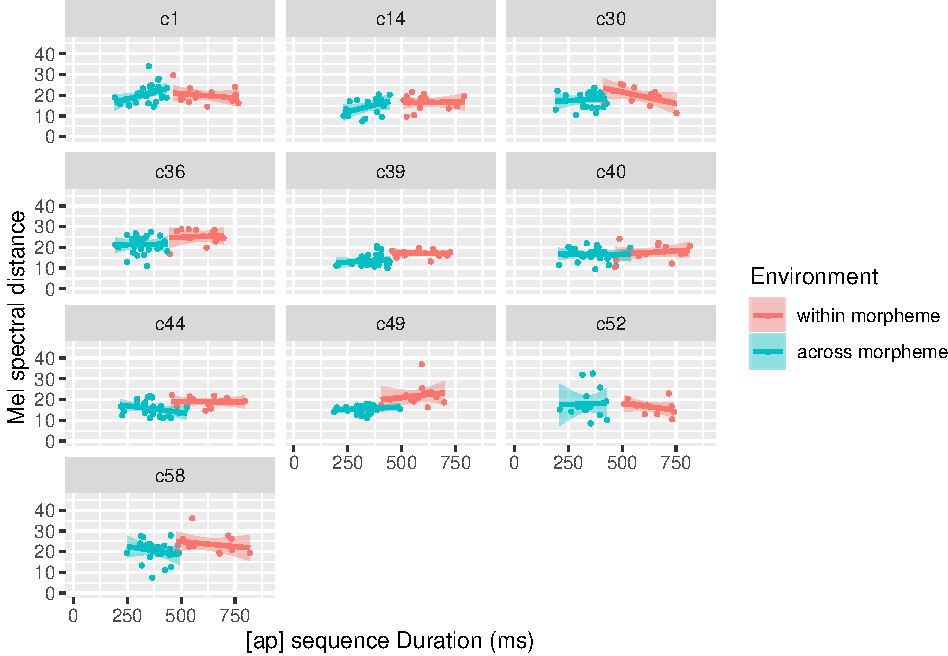
\includegraphics{3_ch3_results_files/figure-latex/five-facet-ap-1.pdf}
\caption{\label{fig:five-facet-ap}Coarticulation by {[}ap{]} duration, word, and morphological environment in five-year-old children}
\end{figure}

\begin{figure}
\centering
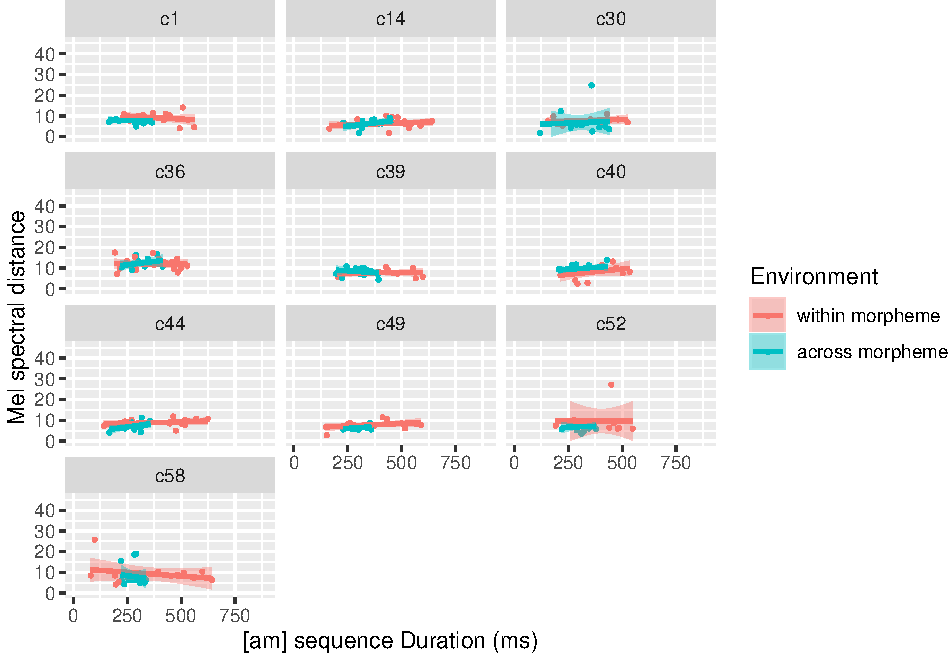
\includegraphics{3_ch3_results_files/figure-latex/five-facet-am-1.pdf}
\caption{\label{fig:five-facet-am}Coarticulation by {[}am{]} duration, word, and morphological environment in five-year-old children}
\end{figure}

\begin{figure}
\centering
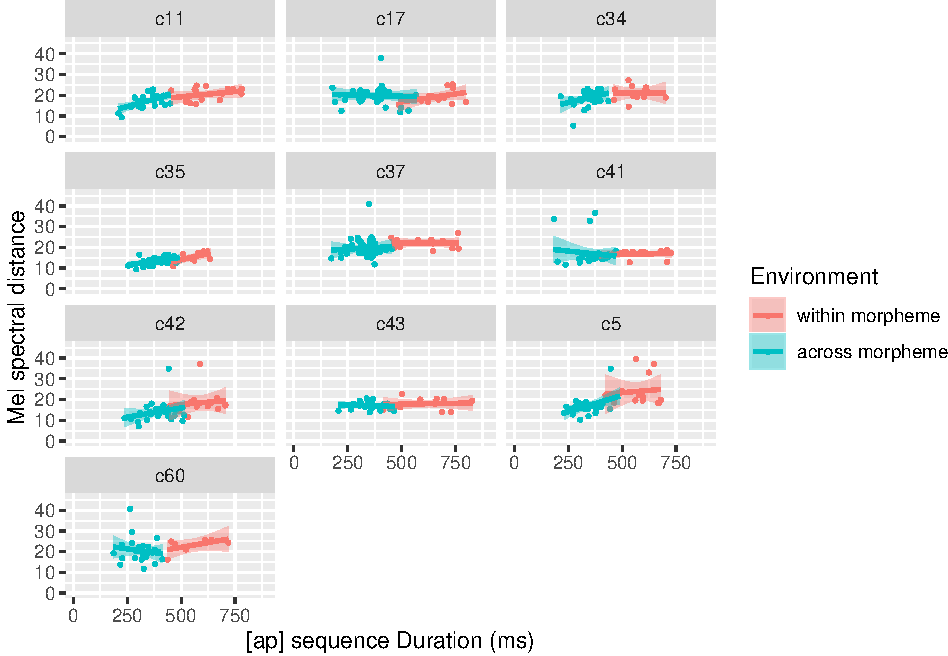
\includegraphics{3_ch3_results_files/figure-latex/six-facet-ap-1.pdf}
\caption{\label{fig:six-facet-ap}Coarticulation by {[}ap{]} duration, word, and morphological environment in six-year-old children}
\end{figure}

\begin{figure}
\centering
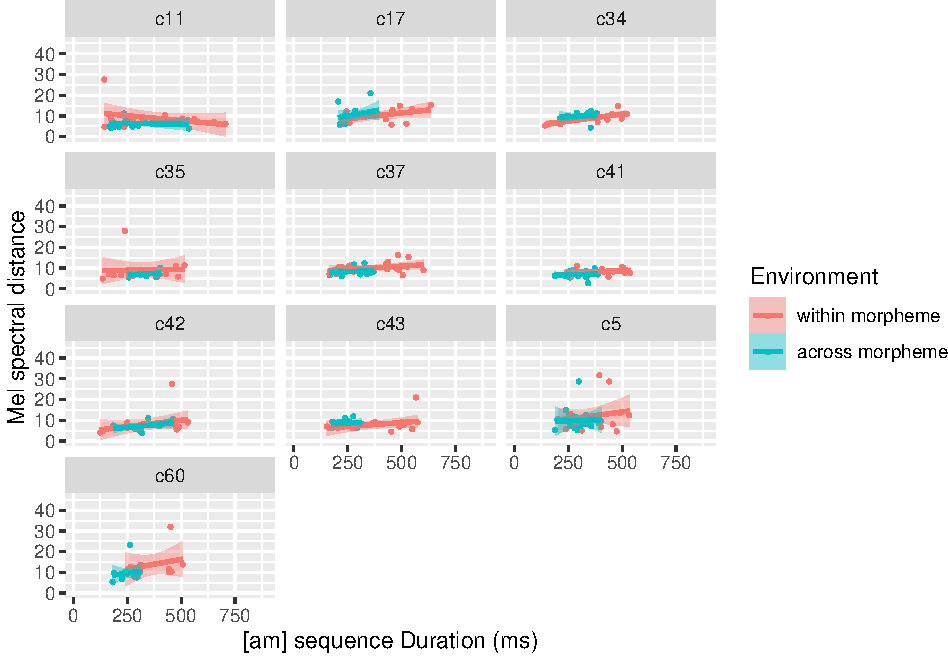
\includegraphics{3_ch3_results_files/figure-latex/six-facet-am-1.pdf}
\caption{\label{fig:six-facet-am}Coarticulation by {[}am{]} duration, word, and morphological environment in six-year-old children}
\end{figure}

\begin{figure}
\centering
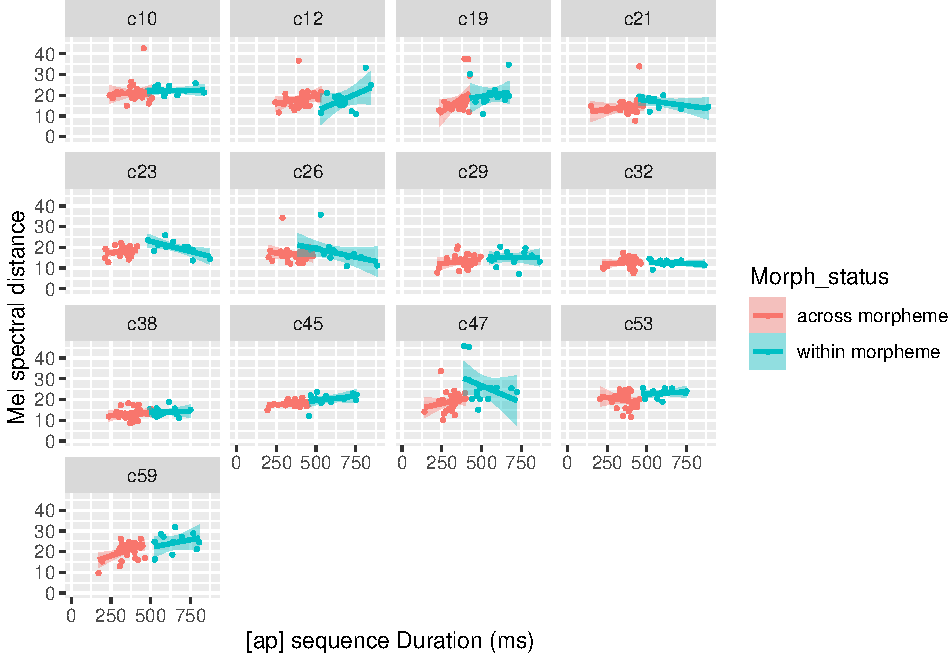
\includegraphics{3_ch3_results_files/figure-latex/seven-facet-ap-1.pdf}
\caption{\label{fig:seven-facet-ap}Coarticulation by {[}ap{]} duration, word, and morphological environment in seven-year-old children}
\end{figure}

\begin{figure}
\centering
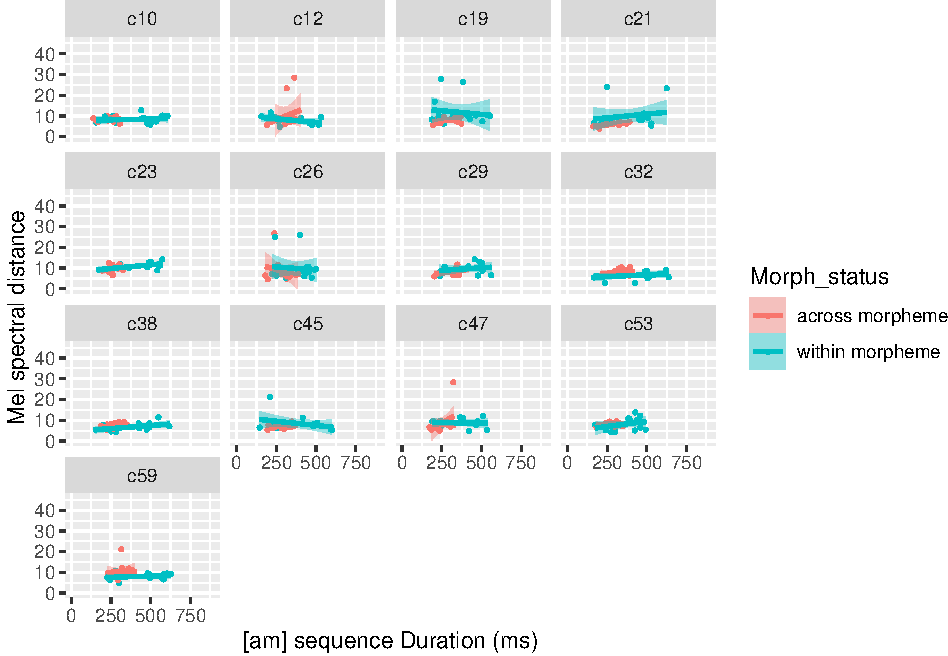
\includegraphics{3_ch3_results_files/figure-latex/seven-facet-am-1.pdf}
\caption{\label{fig:seven-facet-am}Coarticulation by {[}am{]} duration, word, and morphological environment in seven-year-old children}
\end{figure}

\begin{figure}
\centering
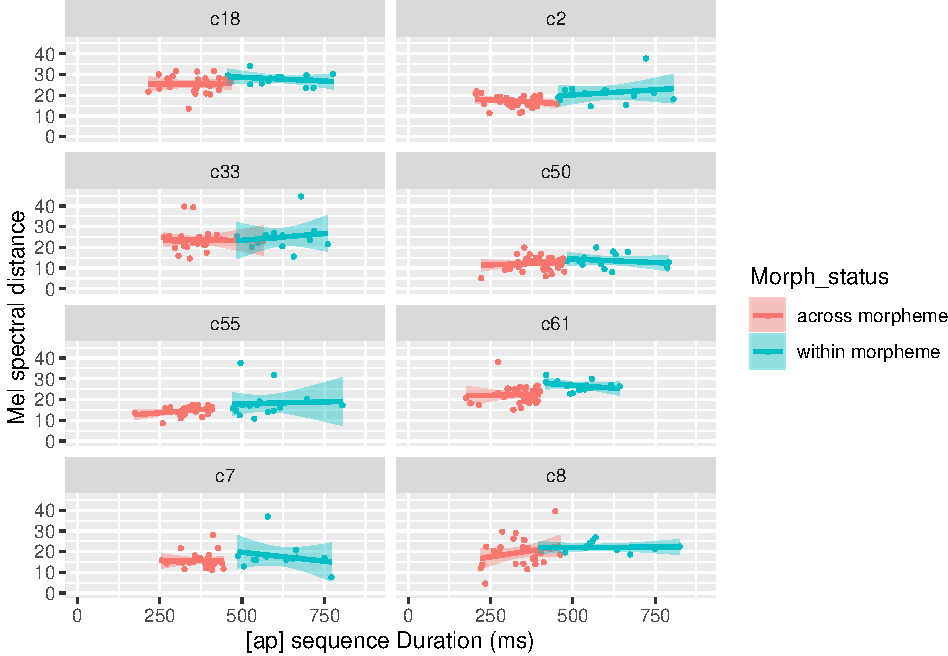
\includegraphics{3_ch3_results_files/figure-latex/eight-facet-ap-1.pdf}
\caption{\label{fig:eight-facet-ap}Coarticulation by {[}ap{]} duration, word, and morphological environment in eight-year-old children}
\end{figure}

\begin{figure}
\centering
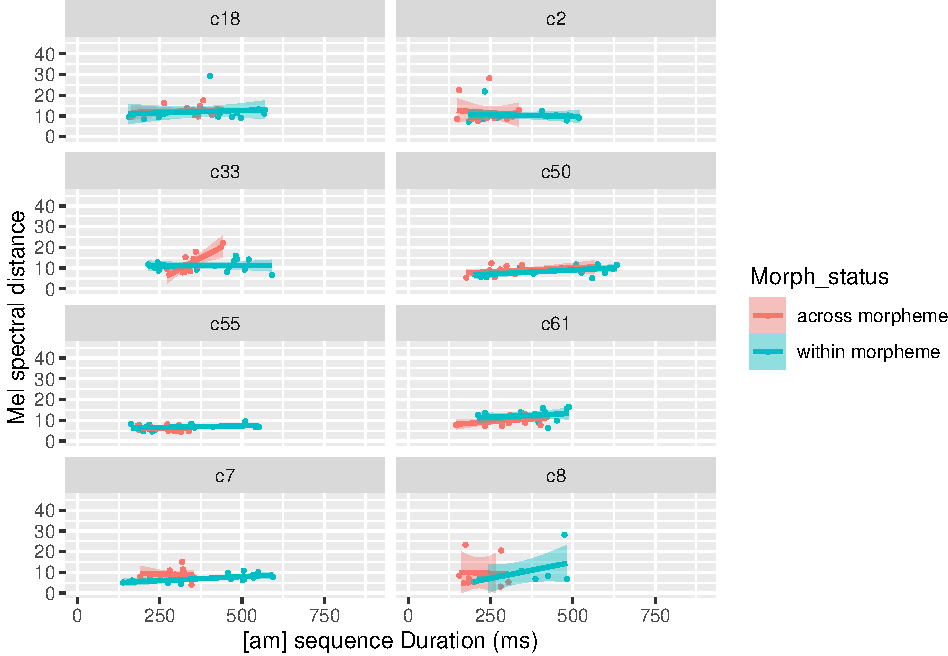
\includegraphics{3_ch3_results_files/figure-latex/eight-facet-am-1.pdf}
\caption{\label{fig:eight-facet-am}Coarticulation by {[}am{]} duration, word, and morphological environment in eight-year-old children}
\end{figure}

\begin{figure}
\centering
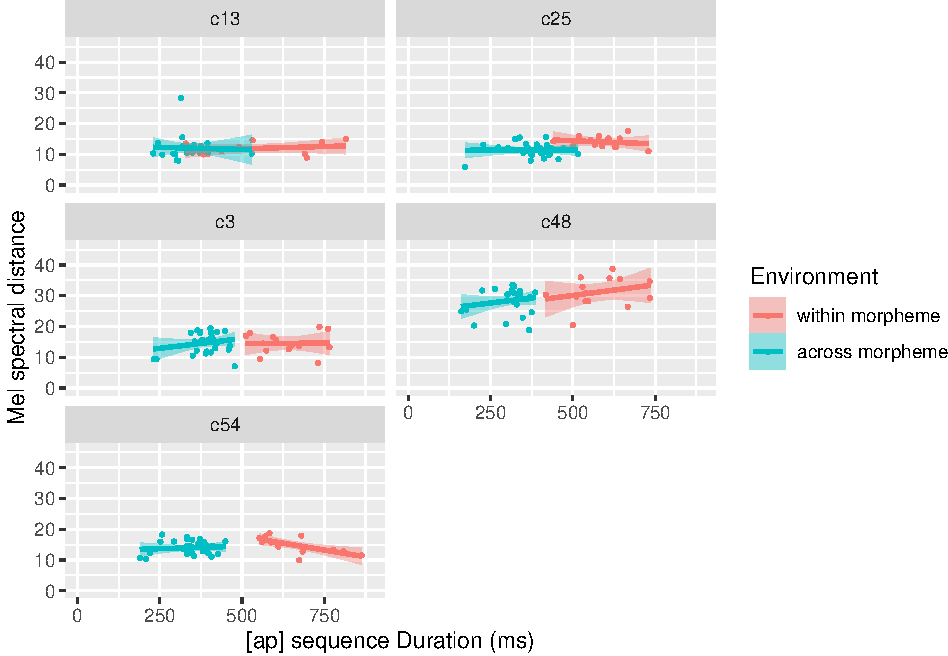
\includegraphics{3_ch3_results_files/figure-latex/nine-facet-ap-1.pdf}
\caption{\label{fig:nine-facet-ap}Coarticulation by {[}ap{]} duration, word, and morphological environment in nine-year-old children}
\end{figure}

\begin{figure}
\centering
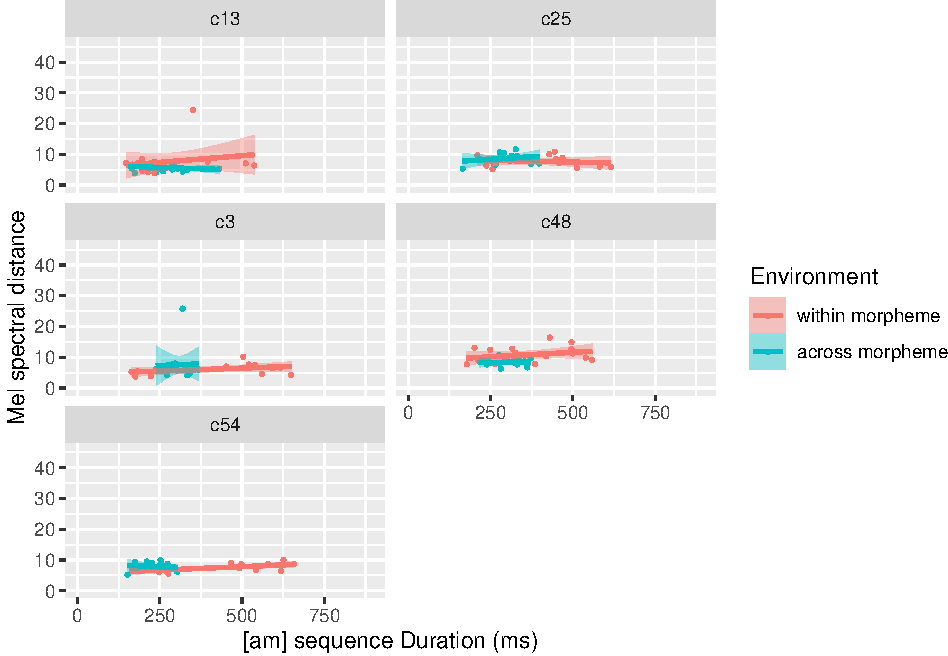
\includegraphics{3_ch3_results_files/figure-latex/nine-facet-am-1.pdf}
\caption{\label{fig:nine-facet-am}Coarticulation by {[}am{]} duration, word, and morphological environment in nine-year-old children}
\end{figure}

\begin{figure}
\centering
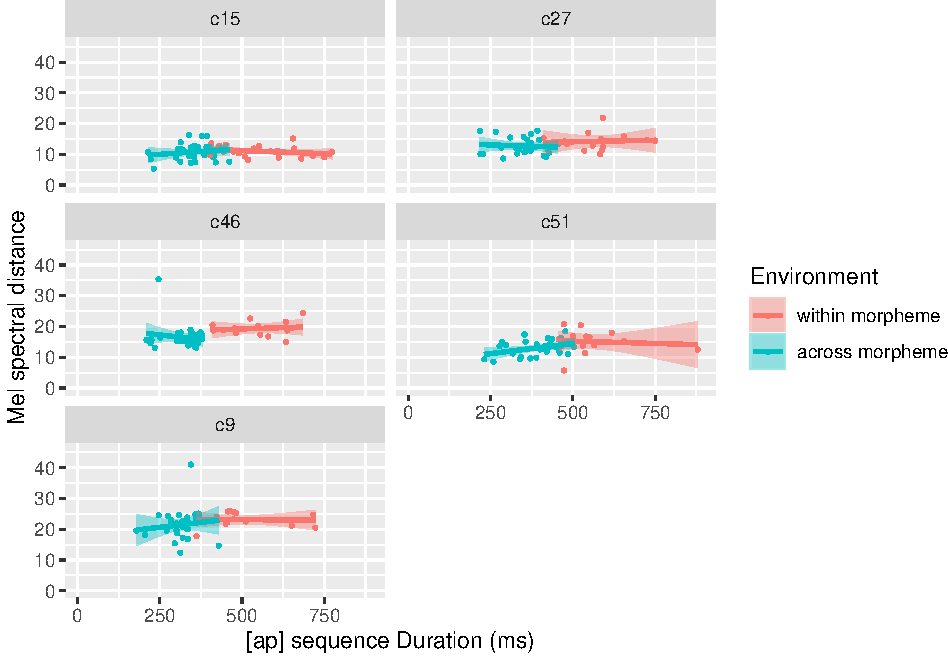
\includegraphics{3_ch3_results_files/figure-latex/ten-facet-ap-1.pdf}
\caption{\label{fig:ten-facet-ap}Coarticulation by {[}ap{]} duration, word, and morphological environment in ten-year-old children}
\end{figure}

\begin{figure}
\centering
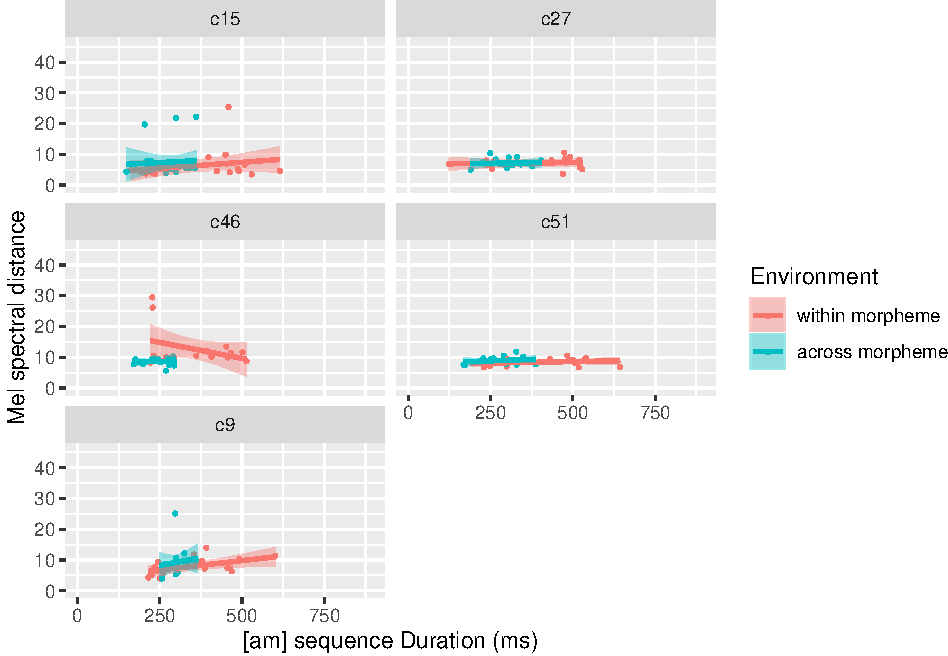
\includegraphics{3_ch3_results_files/figure-latex/ten-facet-am-1.pdf}
\caption{\label{fig:ten-facet-am}Coarticulation by {[}am{]} duration, word, and morphological environment in ten-year-old children}
\end{figure}

\end{document}
